\documentclass{bschlangaul-aufgabe}
\bLadePakete{o-notation}

\usepackage{pgfplots}

\begin{document}
\bAufgabenMetadaten{
  Titel = {Aufgabe 1},
  Thematik = {O-Notation a(), b(), c(), d(), e(n)},
  Referenz = 46115-2021-F.T2-TA2-A1,
  RelativerPfad = Staatsexamen/46115/2021/03/Thema-2/Teilaufgabe-2/Aufgabe-1.tex,
  ZitatSchluessel = examen:46115:2021:03,
  BearbeitungsStand = mit Lösung,
  Korrektheit = unbekannt,
  Ueberprueft = {unbekannt},
  Stichwoerter = {Algorithmische Komplexität (O-Notation)},
  EinzelpruefungsNr = 46115,
  Jahr = 2021,
  Monat = 03,
  ThemaNr = 2,
  TeilaufgabeNr = 2,
  AufgabeNr = 1,
}

\let\O=\bONotationO
\def\of#1{\O{f_#1}}
\def\f#1{$#1(n)$}

\noindent
Sortieren Sie die unten angegebenen Funktionen der O-Klassen \O a, \O b,
\O c, \O d und \O e bezüglich ihrer Teilmengenbeziehungen. Nutzen Sie
ausschließlich die echte Teilmenge $\subsetneq$ sowie die Gleichheit $=$
für die Beziehung zwischen den Mengen. Folgendes Beispiel illustriert
diese Schreibweise für einige Funktionen $f_1$ bis $f_5$. (Diese haben
nichts mit den unten angegebenen Funktionen zu
tun.)\index{Algorithmische Komplexität (O-Notation)}
\footcite{examen:46115:2021:03}

\begin{displaymath}
\of 4 \subsetneq \of 3 = \of 5 \subsetneq \of 1 = \of 2
\end{displaymath}

\noindent
Die angegebenen Beziehungen müssen weder bewiesen noch begründet werden.

\begin{itemize}
\item $a(n) = \sqrt{n^5} + 4n - 5$

\item $b(n) = \log_2 (\log_2(n))$

\item $c(n) = 2^n$

\item $d(n) = n^2 \log(n) + 2n$

\item $e(n) = \frac{4^n}{\log_2n}$
\end{itemize}

\begin{center}
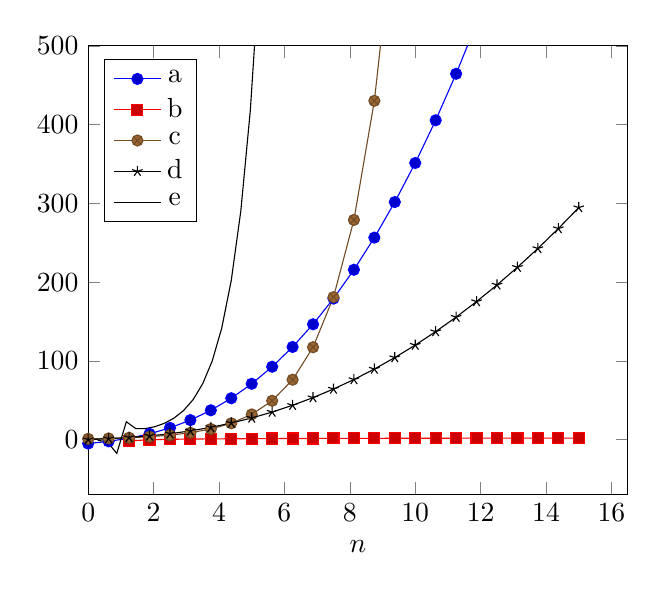
\begin{tikzpicture}
  \begin{axis}[
    xlabel=$n$,
    legend entries={\f a, \f b, \f c, \f d, \f e},
    ymax=500,
    xmin=0,
    legend pos=north west,
    domain=0:15
  ]
  \addplot{sqrt(x^5) + (4 * x) - 5};
  \addplot{log2(log2(x))};
  \addplot{2^x};
  \addplot{x^2 * log10(x) + (2 * x)};
  \addplot[domain=0:7]{4^x / (log2(x))};
\end{axis}
\end{tikzpicture}
\end{center}
\end{document}
